\chapter{Modellek és metrikák kiválasztása}

\section{Kiválasztási és vizsgálati metodika}

A modellek kiválasztásánál elsődleges szempont volt, hogy a különböző mélységi tanulási irányzatok és architekturális paradigmák reprezentálva legyenek. A cél nem pusztán a pontossági versenyeztetés volt, hanem annak megértése is, hogy eltérő típusú architektúrák miként teljesítenek egy valósághű, heterogén, több ezer képből álló, különböző tematikájú képeket tartalmazó adathalmazon (SBphotoThemes180K). A kiválasztott modellek együttesen lefedik:

\begin{itemize}
    \item a klasszikus \textbf{konvolúciós} hálózatokat (pl. \textit{ResNet50}, \textit{Inception-v3}),
    \item a \textbf{sűrű kapcsolatokra építő} architektúrákat (pl. \textit{DenseNet121}),
    \item a \textbf{méretezhető hatékonyságra optimalizált} modelleket (pl. \textit{EfficientNet-B0}),
    \item a \textbf{modern konvolúciós továbbfejlesztéseket} (pl. \textit{ConvNeXt-Tiny}),
    \item a \textbf{transzformer-alapú vizuális feldolgozást} (pl. \textit{ViT-B/16}),
    \item valamint a \textbf{neurális architektúra keresés eredményét} (pl. \textit{NASNet}).
\end{itemize}

Ez a változatosság lehetővé teszi, hogy a vizsgálatokból mélyebb következtetéseket vonjunk le arra vonatkozóan, hogyan skálázhatók, milyen erőforrásigényűek és mennyire robusztusak ezek az architektúrák változatos képi bemenetekkel szemben.

\section{Vizsgált modellek áttekintése és indoklása}

\subsubsection{ResNet50}
A ResNet50 a „Deep Residual Learning” család legismertebb és legszélesebb körben használt tagja. A residual blokk architektúra bevezetésével sikerült megoldani a mély hálózatokban jelentkező gradienseltűnés problémáját. A ResNet egyfajta „alapvonalat” (baseline) is képez, amivel szinte minden új architektúrát össze szoktak vetni, így természetes választás volt a vizsgálathoz.

\textbf{Kategória:} klasszikus konvolúciós hálózat  
\textbf{Fő technológia:} residual kapcsolatok (skip connections), mély konvolúciós blokkok  
\textbf{Miért fontos:} etalonmodell a CNN-ek között, stabil és jól skálázható teljesítmény

\subsubsection{DenseNet121}
A DenseNet egy innovatív megközelítés, amely minden réteget összekapcsol az összes korábbi réteggel (dense connectivity). Ez hatékonyabb információáramlást és gradiens-terjedést biztosít, miközben csökkenti a paraméterszámot a ResNethez képest.

\textbf{Kategória:} sűrű kapcsolású konvolúciós hálózat  
\textbf{Fő technológia:} dense block-ok, átvitt jellemzőtér-bővítés  
\textbf{Miért fontos:} kiváló teljesítmény kisebb hálózati méretek mellett, paraméterhatékony

\subsubsection{EfficientNet-B0}
Az EfficientNet család az architektúrák méretezésének egy új paradigmáját vezette be, ahol a háló mélységét, szélességét és bemeneti felbontását egyidejűleg optimalizálják (compound scaling). Az \textit{B0} verzió a család legkisebb tagja, mégis meglepően jó teljesítményt nyújt alacsony számítási igény mellett.

\textbf{Kategória:} skálázható CNN  
\textbf{Fő technológia:} compound scaling, MBConv blokkok  
\textbf{Miért fontos:} erőforrástakarékos, mégis kiváló pontosságú, ideális mobileszközökre

\subsubsection{ConvNeXt-Tiny}
A ConvNeXt a klasszikus CNN-ek modernizálását célozza, a transzformer architektúrák (főként a Swin Transformer) inspirációival. A ConvNeXt-Tiny modell teljesítményben közel áll a ViT modellekhez, miközben a CNN-ek előnyeit – például hatékony konvolúciót – megőrzi.

\textbf{Kategória:} modern CNN  
\textbf{Fő technológia:} layer normalization, nagyobb kernellek, transzformerszerű blokkok  
\textbf{Miért fontos:} a CNN-ek új generációja, amelyek megközelítik a transzformerek teljesítményét

\subsubsection{ViT-B/16 (Vision Transformer)}
A Vision Transformer a képfeldolgozás egy paradigmaváltó modellje, amely teljesen mellőzi a konvolúciókat. A képet nem pixelenként, hanem patch-enként (16x16) kezeli, és ezekre alkalmaz transzformer blokkokat. Bár hatalmas adatigénye van, érdekes összehasonlítási alapot kínál a CNN-ekhez képest.

\textbf{Kategória:} transzformer-alapú képfeldolgozó modell  
\textbf{Fő technológia:} attention mechanizmus, patch embedding  
\textbf{Miért fontos:} CNN-ek nélküli, tisztán transzformer architektúra; új irány a képfeldolgozásban

\subsubsection{Inception-v3}
Az Inception-v3 a Google által fejlesztett, „Network-in-Network” koncepcióra épülő modell, amely párhuzamosan többféle konvolúciós szűrőt alkalmaz egy rétegen belül. Célja a paraméterhatékonyság és a hálózat komplexitásának optimalizálása.

\textbf{Kategória:} moduláris konvolúciós hálózat  
\textbf{Fő technológia:} inception blokkok, factorized convolutions  
\textbf{Miért fontos:} jól optimalizált, kiegyensúlyozott teljesítmény, mégis alacsony erőforrásigény

\subsubsection{NASNet}
A NASNet (Neural Architecture Search Network) teljesen automatikusan generált architektúra, amely neurális hálózat kereséssel (AutoML) jött létre. Az emberi tervezés helyett algoritmus döntötte el a hálózat blokkjait és struktúráját.

\textbf{Kategória:} automatikusan generált CNN (AutoML)  
\textbf{Fő technológia:} reinforcement learning alapú architektúra keresés  
\textbf{Miért fontos:} betekintést ad az algoritmusok által optimalizált struktúrák előnyeibe és hátrányaiba

\section{Mit tanulhatunk a vizsgálatból?}

Ezen modellek összehasonlítása nemcsak teljesítménybeli különbségekre világít rá, hanem arra is, hogy különböző architektúrák miként kezelik a valósághű, kategória- és témagazdag képi adatokat. A tanulmány során választ kapunk az alábbi kérdésekre:

\begin{itemize}
    \item Mely architektúra típus a leghatékonyabb különböző adatdisztribúciók mellett?
    \item Hogyan teljesítenek a konvolúciós modellek a transzformerekkel szemben?
    \item Érdemes-e automatikusan generált modellekhez nyúlni kézi tervezésű helyett?
    \item Mely modellek mutatnak nagyobb robusztusságot a kisebb elemszámú vagy heterogén kategóriákkal szemben?
\end{itemize}

Ezek megválaszolása elősegíti a jövőbeni adatbázis-építési, modellválasztási és tanítási stratégiák tudatosabb tervezését.

\note{A következő részben szereplő ábrákat saját programból generáltam a torchview draw\_graph könyvtárával. A programkód megtalálható a GitHub repository notebooks/models mappában és a mellékletben.}

\section{Kiválasztott modellek részletes ismertetése}

\subsection{ResNet50}

\begin{figure}[H]
    \centering
    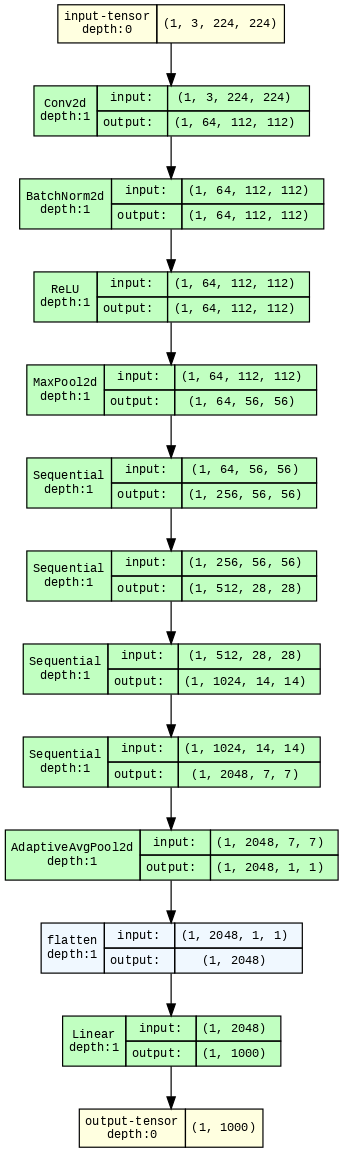
\includegraphics[width=0.4\textwidth]{images/models/ResNet50_overview.png}
    \caption{A ResNet50 szerkezete.}
    \label{fig:ResNet50_overview}
\end{figure}

A \textbf{ResNet50} (Residual Network, 50 réteg mélységű változat) az egyik legmeghatározóbb konvolúciós neurális hálózat, amelyet a Microsoft Research mutatott be 2015-ben a Deep Residual Learning for Image Recognition című tanulmányban \cite{article_resnet50}. Az innováció lényege az ún. \textit{residual blokk}, amely lehetővé teszi a gradiens hatékony terjedését mély rétegeken keresztül.

\paragraph{Működési elve:} A ResNet az identitástér leképezését támogatja azáltal, hogy ún. \textit{skip connection}-öket használ, azaz az inputot változatlanul átadja több rétegen keresztül. Ezzel megelőzi a tanulási nehézségeket, amelyek mély hálók esetén jelentkeznek (pl. gradiens eltűnés, torzulás).

\paragraph{Felépítése:} A ResNet50 50 konvolúciós rétegből áll, melyek \textit{bottleneck} struktúrákba rendeződnek: egy $1\times1$, egy $3\times3$ majd újra egy $1\times1$ konvolúciót tartalmaz minden blokk. Az így kialakított architektúra mély, de mégis hatékonyan tanítható.

\paragraph{Előnyei:}
\begin{itemize}
    \item Rendkívül mély hálózat is stabilan tanítható
    \item Széles körben elérhető előtanított súlyok
    \item Jól működik sokféle feladaton, „baseline”-modellként is tekinthető
\end{itemize}

\paragraph{Hátrányai:}
\begin{itemize}
    \item Nagyobb memóriaigény, főleg inference során
    \item A későbbi, modernebb architektúrákhoz képest nem optimális hatékonyság
\end{itemize}

A ResNet50 tehát egy rendkívül erős és megbízható kiindulópont, amely kiváló összehasonlítási alapként szolgálhat más, újabb modellek értékelésekor.

\subsection{DenseNet121}

\begin{figure}[H]
    \centering
    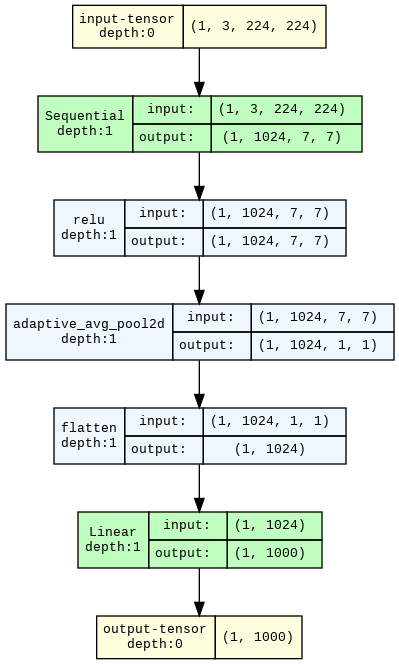
\includegraphics[width=0.4\textwidth]{images/models/DenseNet121_overview.png}
    \caption{A DenseNet121 szerkezete.}
    \label{fig:DenseNet121_overview}
\end{figure}

A \textbf{DenseNet121} (Densely Connected Convolutional Network) szintén egy mély konvolúciós architektúra, amelyet 2017-ben mutattak be \cite{article_densenet}. A DenseNet fő újítása az, hogy minden réteg bemenete az összes korábbi réteg kimenetét is tartalmazza. Ez a „sűrű kapcsolódás” (dense connectivity) elméletileg és gyakorlatilag is javítja az információáramlást és a tanulást.

\paragraph{Működési elve:} A DenseNet nem egyszerűen egymásra épülő rétegeket tartalmaz, hanem minden réteg minden korábbi réteg kimenetét megkapja inputként. Ezáltal az információ és a gradiens nagyon hatékonyan tud terjedni a hálózatban, és kevésbé fordul elő információvesztés.

\paragraph{Felépítése:} A DenseNet121 négy dense blokkot tartalmaz, melyek között ún. \textit{transition} rétegek találhatók, ezek csökkentik a méretet és a csatornaszámot. Az architektúra 121 mély rétegből áll, de a sűrű kapcsolódás miatt a paraméterszáma jóval alacsonyabb, mint a ResNet50-é.

\paragraph{Előnyei:}
\begin{itemize}
    \item Magas hatékonyság kis paraméterszámmal
    \item Kiváló gradiens- és információáramlás
    \item Jó generalizációs képesség, főleg kis adathalmazoknál
\end{itemize}

\paragraph{Hátrányai:}
\begin{itemize}
    \item Lassabb tanítás, mivel sok kapcsolatot kell kezelni
    \item Nagyobb memóriahasználat az összesített rétegbemenetek miatt
\end{itemize}

A DenseNet121 különösen hasznos olyan feladatoknál, ahol fontos a finom részletek megőrzése és hatékony gradiensáramlás, ugyanakkor a paraméterhatékonyság is számít.

\subsection{EfficientNet-B0}

\begin{figure}[H]
    \centering
    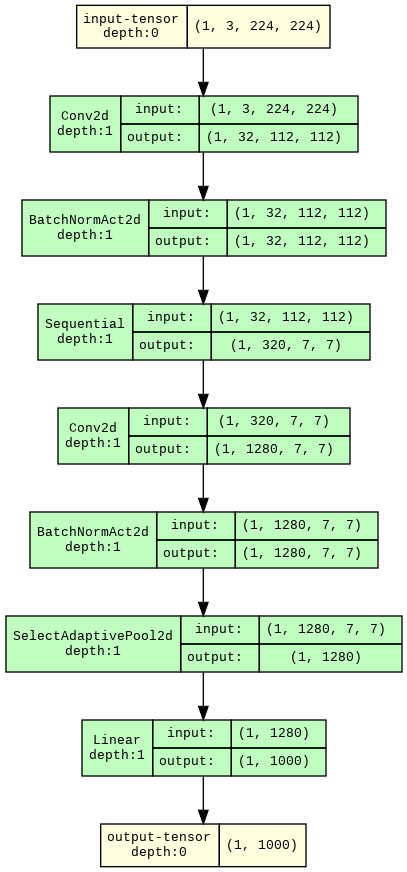
\includegraphics[width=0.4\textwidth]{images/models/EfficientNet-B0_overview.png}
    \caption{A EfficientNet-B0 szerkezete.}
    \label{fig:EfficientNet-B0_overview}
\end{figure}

Az \textbf{EfficientNet-B0} a Google Brain által bemutatott EfficientNet család legalapvetőbb és legkisebb változata \cite{article_efficientnet}. A család célja a hálózati méretezés (scaling) szisztematikus, egységesített megközelítése, amely egyszerre optimalizálja a mélységet, szélességet és felbontást egy ún. „compound scaling” képlettel.

\paragraph{Működési elve:} Ahelyett, hogy egyetlen dimenzió mentén növelnénk a háló méretét (mint pl. csak mélység vagy csak szélesség), az EfficientNet minden dimenziót együtt skáláz a legjobb hatékonyság elérése érdekében. Az alapot egy optimalizált NASNet-féle „mobilbarát” blokk, az \textit{MBConv} adja, amely depthwise separable convolutions-t használ.

\paragraph{Felépítése:} Az EfficientNet-B0 7 MBConv-blokk szintből áll, amelyek kombinálják a bővített konvolúciókat (expansion), depthwise konvolúciót és squeeze-and-excitation (SE) modulokat. Mindez együtt egy kompakt, de rendkívül hatékony architektúrát eredményez.

\paragraph{Előnyei:}
\begin{itemize}
    \item Kiemelkedő pontosság alacsony számítási költségek mellett
    \item Ideális mobil- vagy beágyazott rendszerekre
    \item Modern méretezési elv, amelyet az egész család kiterjeszt
\end{itemize}

\paragraph{Hátrányai:}
\begin{itemize}
    \item Az MBConv blokkok miatt nehezebben értelmezhető, „black-box” jellege lehet
    \item A kis modellváltozatok érzékenyebbek a bemeneti adatok minőségére
\end{itemize}

Az EfficientNet-B0 egy remek választás minden olyan környezetben, ahol fontos a hatékonyság, de nem akarunk kompromisszumot kötni a pontosság terén.

\subsection{ConvNeXt-Tiny}

\begin{figure}[H]
    \centering
    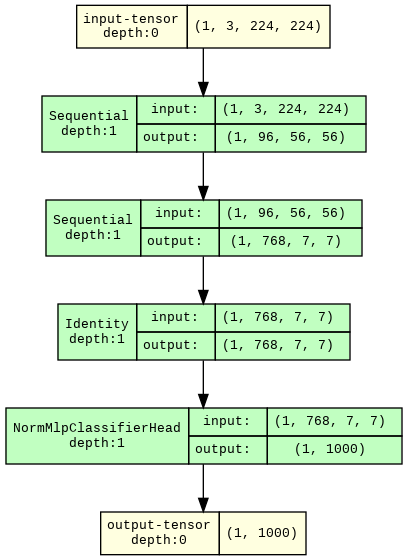
\includegraphics[width=0.4\textwidth]{images/models/ConvNeXt-Tiny_overview.png}
    \caption{A ConvNeXt-Tiny szerkezete.}
    \label{fig:ConvNeXt-Tiny}
\end{figure}

A \textbf{ConvNeXt-Tiny} a 2022-ben bemutatott ConvNeXt architektúra legkisebb változata, amely a konvolúciós neurális hálózatokat (\textit{CNN}) modernizálja a Vision Transformer (ViT) modellek elveinek figyelembevételével \cite{article_convnext}. A cél az volt, hogy újra felélesszék a CNN-ek relevanciáját a transformer-alapú modellek dominanciájával szemben, különösen a számítástechnikai hatékonyság szempontjából.

\paragraph{Működési elve:} A ConvNeXt megőrzi a klasszikus konvolúciós rétegek használatát, de számos architekturális újítást alkalmaz: például normalizációk sorrendje, nagyobb kernelméretek ($7\times7$), LayerNorm használata BatchNorm helyett, és az aktivációk újraértelmezése. Ezek az elemek kombinálva adják az „evolved CNN” karaktert.

\paragraph{Felépítése:} A „Tiny” változat négy szintű hierarchiát alkalmaz, összesen 28 blokkal, és mindössze 28 millió paraméterrel. Az architektúra hatékony és méretében optimalizált, kimondottan jól teljesít kis számítási költségű környezetekben is.

\paragraph{Előnyei:}
\begin{itemize}
    \item Megőrzi a CNN-ek hatékonyságát, de modern ViT-ihlette frissítésekkel
    \item Kompakt modell – gyors tanítás és alacsony memóriaigény
    \item Kimagasló teljesítmény ViT szintjén, de egyszerűbb tanítási folyamat
\end{itemize}

\paragraph{Hátrányai:}
\begin{itemize}
    \item Még viszonylag új architektúra – kevesebb ipari alkalmazás és benchmark
    \item A ViT-nél kisebb képesség a hosszú távú kapcsolatok felismerésére
\end{itemize}

A ConvNeXt-Tiny ideális választás minden olyan feladathoz, ahol a legkorszerűbb CNN-technológia hatékonysága és egyszerűsége is előnyt jelent.

\subsection{ViT-B/16}

\begin{figure}[H]
    \centering
    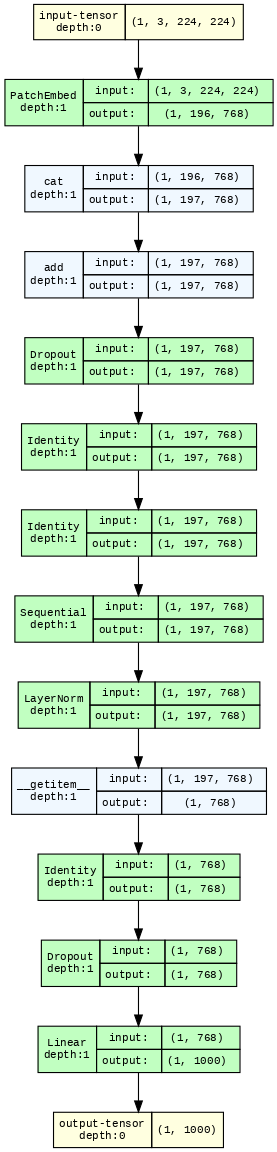
\includegraphics[width=0.2\textwidth]{images/models/ViT-B16_overview.png}
    \caption{A ViT-B/16 szerkezete.}
    \label{fig:B16_overview}
\end{figure}

A \textbf{Vision Transformer Base/16} (röviden \textbf{ViT-B/16}) az első, széles körben elismert \textit{pure transformer} architektúra, amely képeket dolgoz fel a természetes nyelvfeldolgozásban használt transformer architektúra átalakításával \cite{article_vit_b16}. A modell a képeket fix méretű patch-ekre bontja, és ezeket a patch-eket sorozatként kezeli, hasonlóan a szavakhoz egy nyelvi modellben.

\paragraph{Működési elve:} A ViT modellek nem használnak konvolúciókat. Ehelyett a képeket $16\times16$ pixeles foltokra bontják, amelyek lineáris rétegen keresztül kerülnek embed-elésre. Ezután klasszikus transformer encoder blokkok következnek – többfejű figyelemmel (multi-head attention) és feed-forward rétegekkel.

\paragraph{Felépítése:} A ViT-B/16 12 transformer blokkból áll, összesen 86 millió paraméterrel. A „/16” azt jelenti, hogy a bemenet $16\times16$ pixeles foltokra van osztva. A képeket egy „class token” egészíti ki, amelyre a végső predikció épül.

\paragraph{Előnyei:}
\begin{itemize}
    \item Kiváló hosszú távú kapcsolat-érzékelő képesség
    \item Skálázhatóság – nagyobb modellekkel arányosan nő a teljesítmény
    \item Egyszerű, elegáns architektúra konvolúciók nélkül
\end{itemize}

\paragraph{Hátrányai:}
\begin{itemize}
    \item Nagy adatmennyiséget igényel a hatékony tanuláshoz
    \item Lassabb konvergencia, érzékenyebb a hiperparaméterekre
    \item Kevésbé hatékony kis modellek és kisebb adathalmazok esetén
\end{itemize}

A ViT-B/16 segítségével összehasonlítható, hogy a „pure attention” alapú modellek hogyan teljesítenek a klasszikus és új generációs CNN-ekhez képest.

\subsection{Inception-v3}

\begin{figure}[H]
    \centering
    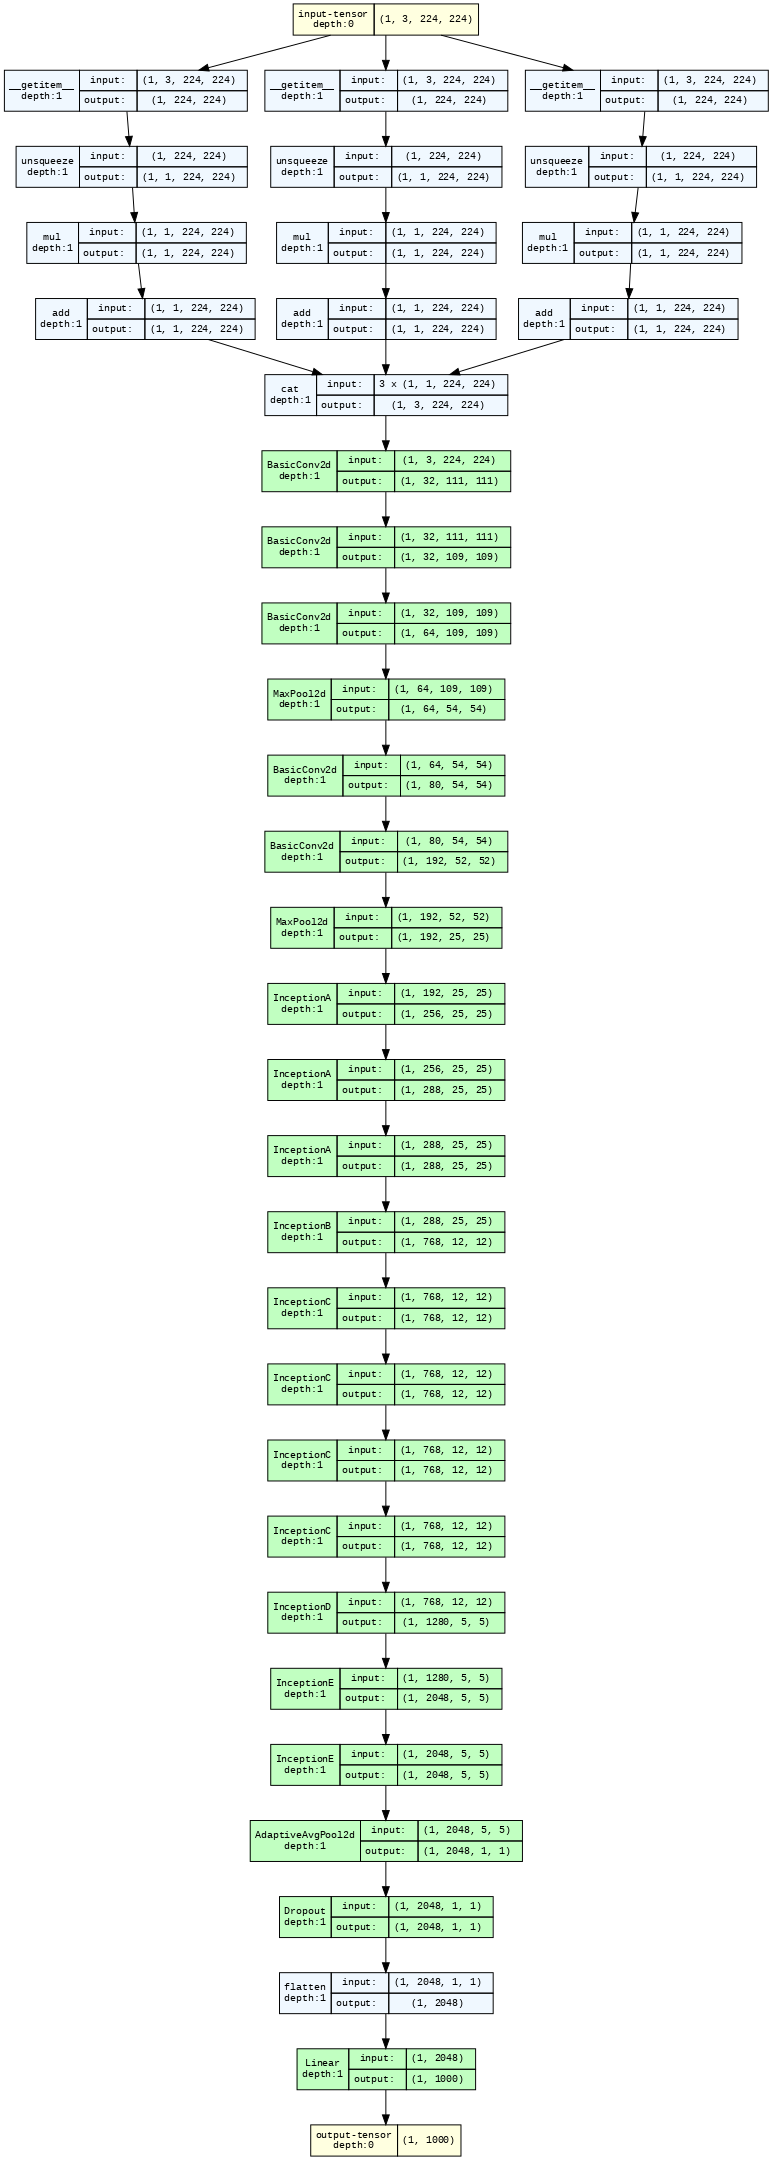
\includegraphics[width=0.35\textwidth]{images/models/Inception-v3_overview.png}
    \caption{A Inception-v3 szerkezete.}
    \label{fig:Inception-v3_overview}
\end{figure}

Az \textbf{Inception-v3} a Google által fejlesztett Inception-sorozat egyik legnépszerűbb és legsikeresebb verziója, amelyet 2015-ben mutattak be \cite{article_inception_v3}. A fő cél a számítási hatékonyság növelése anélkül, hogy csökkenne a pontosság. Az architektúra újdonsága az Inception-modul, amely különböző méretű konvolúciókat párhuzamosan futtat, így több skálán is képes információt kinyerni.

\paragraph{Működési elve:} Az Inception-v3 egy összetett architektúra, amelyben a konvolúciós rétegeket párhuzamosan, különböző szűrőméretekkel (pl. $1\times1$, $3\times3$, $5\times5$) alkalmazzák, és ezek kimenetét egyesítik. Ez lehetővé teszi a hatékony, mély és széles jellemzők kinyerését különböző felbontásokon.

\paragraph{Felépítése:} A hálózat több Inception-modulból áll, melyek között redukciós (méretcsökkentő) blokkok találhatók. A teljes modell körülbelül 24 millió paraméterből áll, ami viszonylag kis szám az akkori modellekhez képest.

\paragraph{Előnyei:}
\begin{itemize}
    \item Hatékony architektúra – kevesebb paraméter, mégis magas pontosság
    \item Több skálán történő reprezentációtanulás
    \item Jó választás korlátozott erőforrások mellett is
\end{itemize}

\paragraph{Hátrányai:}
\begin{itemize}
    \item Bonyolultabb architektúra, nehezebb reprodukálni
    \item A későbbi modellek hatékonyabban kihasználják a modern hardvereket
\end{itemize}

Az Inception-v3 egy történetileg fontos, hatékony CNN-architektúra, amely értékes összehasonlítási alap a modernebb, komplexebb modellekhez képest.

\subsection{NASNet}

\begin{figure}[H]
    \centering
    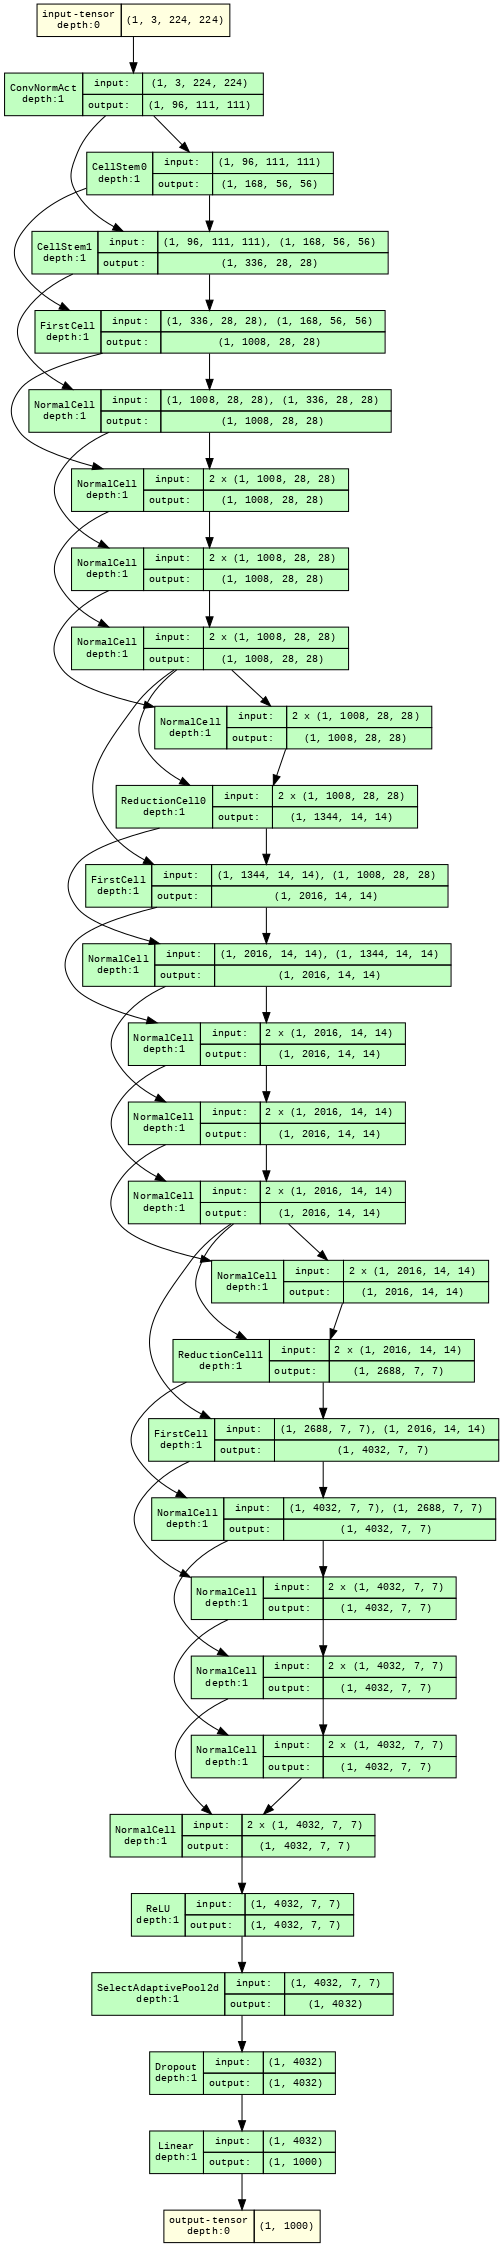
\includegraphics[width=0.25\textwidth]{images/models/NASNet_overview.png}
    \caption{A NASNet szerkezete.}
    \label{fig:NASNet_overview}
\end{figure}

A \textbf{NASNet} (Neural Architecture Search Network) egy olyan architektúra, amelyet nem ember, hanem gépi tanulás által optimalizált keresőalgoritmus (NAS – Neural Architecture Search) hozott létre. A Google AutoML csapata mutatta be 2018-ban \cite{article_nasnet}. A cél az volt, hogy automatikusan találjanak kiemelkedően teljesítő neurális hálóarchitektúrákat.

\paragraph{Működési elve:} A NASNet modulokat kis, ismétlődő „cellákra” bontják: egy „normal cell”-re és egy „reduction cell”-re. Ezeket egy keresőalgoritmus iteratívan optimalizálja egy kisebb adathalmazon (pl. CIFAR-10), majd a végső architektúrát átméretezik a célfeladathoz (pl. ImageNet).

\paragraph{Felépítése:} A NASNet nagyméretű, moduláris modell, amely tipikusan 88 millió paramétert tartalmaz a „NASNet-A Large” változatban, de léteznek kisebb, mobilos verziók is (pl. NASNet-Mobile).

\paragraph{Előnyei:}
\begin{itemize}
    \item Automatikus optimalizálás – gyakran jobb eredmények emberi tervezés nélkül
    \item Moduláris, skálázható architektúra
    \item Jó teljesítmény mind számításigényes, mind mobil környezetben
\end{itemize}

\paragraph{Hátrányai:}
\begin{itemize}
    \item Komplex tanítási folyamat – a NAS futtatása rendkívül erőforrás-igényes
    \item Nehezebben interpretálható, mint a kézzel tervezett modellek
\end{itemize}

A NASNet betekintést enged az architektúra-keresésen alapuló modern modellek világába, és összehasonlítási lehetőséget nyújt az ember által tervezett modellekkel szemben.


\section{A kiválasztott metrikák}

A modellek kiértékelése során olyan metrikák alkalmazása szükséges, amelyek átfogó és megbízható képet adnak a tanítás hatékonyságáról, a generalizációs képességekről, valamint az adott feladathoz való illeszkedésről. A kiválasztott metrikák jól bevált, nemzetközileg elismert szabványok a számítógépes látás és osztályozási feladatok körében. A következőkben részletesen ismertetem ezen metrikák jelentését és indoklását.

\subsection{Top-1 pontosság}

A \textbf{Top-1 pontosság} azt méri, hogy a modell legnagyobb valószínűséggel megjósolt osztálya megegyezik-e a valódi címkével. Ez a leggyakoribb és legegyszerűbb értékelési mód képosztályozási feladatok esetén. Különösen fontos, amikor a cél az, hogy a modell első próbálkozásra pontosan eltalálja a helyes kategóriát.

\textit{Miért választottam?}  
Mivel az alkalmazás célja pontos osztályozás, ezért elengedhetetlen látni, hogy az elsődleges (legvalószínűbb) predikciók milyen mértékben feleltethetők meg a valóságos címkéknek.

\subsection{Top-5 pontosság}

A \textbf{Top-5 pontosság} azt vizsgálja, hogy a modell által megjósolt öt legvalószínűbb kategória között szerepel-e a helyes válasz. Ezt gyakran használják olyan osztályozási problémáknál, ahol sok a hasonló kategória (pl. madárfajok, járműtípusok), és a teljesen pontos becslés helyett a „jó irány” is informatív.

\textit{Miért választottam?}  
Mivel az SBphotoThemes180K adathalmazban számos átfedő és vizuálisan hasonló kategória található, a Top-5 pontosság segít feltárni, ha a modell ugyan nem találja el elsőre a helyes kategóriát, de erősen közelíti azt.

\subsection{Precision}

A \textbf{precision} (pozitív predikciós érték) megmutatja, hogy az adott osztályra vonatkozóan a modell által „pozitívnak” vélt találatok közül hány volt valóban helyes. Ez fontos ott, ahol a téves pozitív eredmények költségesek lehetnek.

\textit{Miért választottam?}  
Ez a metrika különösen hasznos annak vizsgálatára, hogy mennyire „megalapozottak” a modell predikciói: azaz, ha a modell valamit „biztosra” mond, az milyen arányban bizonyul igaznak.

\subsection{Recall}

A \textbf{recall} (érzékenység) azt mutatja meg, hogy az adott osztályba tartozó valódi példányok közül mennyit ismer fel a modell. Ez akkor fontos, ha nem akarunk elvéteni fontos eseteket (pl. egészségügyi vagy biztonsági alkalmazásokban).

\textit{Miért választottam?}  
Segít annak feltérképezésében, hogy a modell mennyire képes felismerni az adott osztályba tartozó képeket, még akkor is, ha azok eltérnek a tipikus mintától.

\subsection{F1-score}

Az \textbf{F1-score} a precision és a recall harmonikus átlaga. Ez kiegyensúlyozott mérőszám, amely akkor is informatív, ha a két előző mutató eltérő tendenciát mutat.

\textit{Miért választottam?}  
Az F1-score révén egyetlen értékben kaphatunk képet a modell általános osztályozási képességéről, figyelembe véve mind a túlzott pozitív predikciókat, mind a kihagyott eseteket.

\subsection{Train és Val loss}

A \textbf{train loss} és a \textbf{validation loss} a modell tanítása során keletkező veszteség (loss function értéke) alakulását mutatja. A train loss a tanítóhalmazon, míg a val loss az ismeretlen validációs adatokon mért érték.

\textit{Miért választottam?}  
Ezek elengedhetetlen metrikák a tanulási folyamat nyomon követéséhez. A két görbe összehasonlításával feltárható a modell túlilleszkedése (\textit{overfitting}) vagy alulilleszkedése (\textit{underfitting}).

\subsection{Train és Val pontosság}

A \textbf{train accuracy} és a \textbf{validation accuracy} megmutatják, hogy a modell milyen arányban jósolja meg helyesen a címkéket a tanító, illetve a validációs halmazon. Ezek értéke szorosan összefügg a loss értékekkel, de intuitívabbak és könnyebben értelmezhetők.

\textit{Miért választottam?}  
A pontosság segít vizuálisan és numerikusan követni a tanítás sikerességét. Az eltérés a tanító és a validációs pontosság között utalhat az általánosító képesség hiányosságaira.

\section{Összegzés}

Ebben a fejezetben részletesen bemutattam azokat a mélytanulási modelleket, amelyeket az SBphotoThemes180K adathalmaz osztályozási teljesítményének értékelésére kiválasztottam. A modellek között megtalálhatók a klasszikus konvolúciós architektúrák, mint a ResNet50 és az Inception-v3, a paraméterhatékonyságra optimalizált megközelítések, mint az EfficientNet-B0 és a NASNet, valamint a korszerűbb, transzformer-alapú ViT-B/16 modell és a ConvNeXt, amely a modern ViT-hatásokkal bővített konvolúciós architektúrák új hullámát képviseli.

A modellek kiválasztását indokolja az, hogy különböző architekturális iskolákat képviselnek, eltérő számítási igénnyel, parametrikus komplexitással és általánosító képességgel rendelkeznek. Ez lehetővé teszi a mély tanulási megközelítések közötti összehasonlítást egy viszonylag nagy, valóságból származó képadatbázison.

A teljesítmény értékeléséhez használt metrikák szintén tudatos választás eredményei: a Top-1 és Top-5 pontosság alapvető osztályozási mutatók, míg a Precision, Recall és F1-score lehetővé teszik az egyensúlyi hibák feltérképezését, különösen sokosztályos feladatoknál. A tanulási folyamat megértéséhez és optimalizálásához pedig a loss és pontosság alakulásának idősoros vizsgálata szolgál alapul.

Ezen modellek és metrikák együttes vizsgálata biztosítja, hogy a későbbi fejezetekben bemutatott kísérleti eredmények nemcsak technikai szempontból megalapozottak, hanem mélyebb következtetések levonására is alkalmasak a modellválasztás, az architektúra-hatékonyság, valamint az adathalmaz minőségének és nehézségi szintjének szempontjából.